\noindent In this doctoral thesis I have presented three searches for new, heavy resonances decaying to two vector bosons in the all-hadronic final state, using datasets collected by the CMS experiment corresponding to an integrated luminosity of 2.7 (2015), 35.9 (2016) and 77.3 (2016+2017) \fbinv. Due to the high energy ("boost") of the vector bosons, their decay products are so collimated that they get merged into one single jet, leading to a dijet final state topology.
Dedicated jet grooming and jet substructure techniques are therefore explored in order to discriminate vector bosons from the overwhelming QCD multijet background. \par
Each of the analyses presented has provided original contributions to the field: the first search was the first of its kind to ever be performed at $\sqrt{\rm{s}}=13 \TeV$, following an observed excess of 3.4 (1.3) $\sigma$ by ATLAS (CMS) in the 8 \TeV dataset, and the first time CMS demonstrated the efficiency of using jet-grooming techniques at trigger level. It, at the time, set the most stringent limits to date for the signal scenarios under consideration. The second search introduces a novel pileup-resistant and perturbative-safe vector boson tagging algorithm based on using PUPPI for pileup subtraction, and softdrop for jet grooming, ensuring a high and stable signal efficiency up to a pileup of at least 50 interactions per event. The optimization, validation, and full commissioning of the tagger was performed in the context of this search. Dedicated jet mass corrections, in order to account for an observed \PT and $\eta$ dependence in PUPPI softdrop jet mass, due to the nature of the softdrop algorithm, were also developed. The tagger based on PUPPI with softdrop, together with the jet mass corrections, became, and still is, the recommended algorithm for W-tagging in CMS. \par
The final analysis introduces a brand new way of doing diboson resonance searches through a three-dimensional fit of the dijet invariant mass and the masses of the two jets. By optimizing the W-tagging algorithm used in this search and due to the nature of the search method, we have, for the first time, been able to constrain the jet mass scale and resolution from a boosted  $\PW(\bar{\rm{q}}\rm{q})$ and $\PZ(\bar{\rm{q}}\rm{q})$ peak produced by the V+jets standard model process. The method itself leads to a 20-30 \% higher sensitivity than the default search method.\par
The benefit of using a three-dimensional fit based on dijet invariant mass and the masses of the two jets, is that one can look for resonances peaking anywhere in the jet mass and dijet invariant mass spectrum. The natural next step for this search is therefore the incorporation of VH(bb) and H(bb)H(bb) final states into the three-dimensional fit framework, where orthogonality is guaranteed through b-tagging categories. This process is ongoing and planned for the full Run 2 dataset (including the data collected in 2018).\newline
Going further, one can incorporate searches for generic resonances peaking anywhere in the softdrop jet mass and dijet invariant mass spectrum in the multi-dimensional fit, where the jets themselves can have substructure compositions other than two subjets. This type of model-independent search requires a generic anti-QCD tagger in order to be truly model independent. \par
In the final chapter of this thesis I presented ongoing work on a on a W-tagging algorithm using a deep neural network for future searches, capable of more than doubling the analysis signal efficiency by incorporating jet substructure algorithms within the deep layers. As there will be no center-of-mass energy increase after the LHC reaches 14 \TeV, achieving the best possible analysis sensitivity for the dataset to come will be of key importance. I also showed how such a deep neural network model is the ideal starting point for building a signal-independent anti-QCD tagger. With $\sim80$ \fbinv of 13 \TeV data analyzed and no excess observed, the future of this search therefore lies in increasing the analysis sensitivity through novel taggers, as the one I have presented here, and, making the search strategy as generic as possible through multi-dimensional scans and generic anti-QCD taggers, both of which have a foundation now built within this doctoral work.
\begin{figure}[b!]
\centering
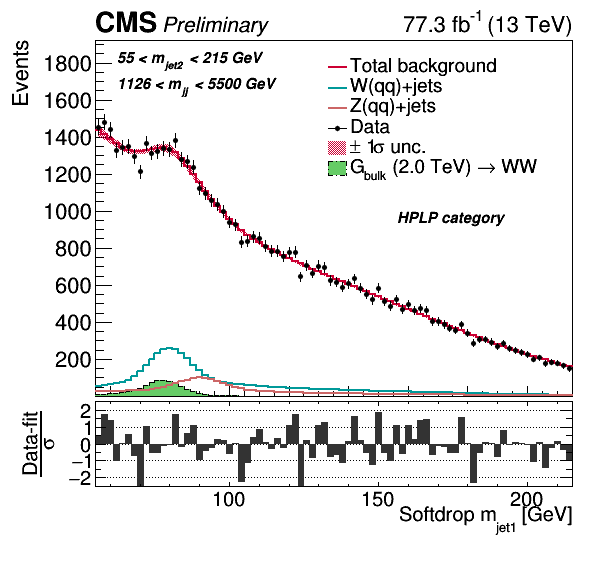
\includegraphics[width=0.69\textwidth]{figures/analysis/search3/AN-17-303/postfitchecks/postfit_HPLP_unblind/PostFitComboHPLP_X-Proj__y___0_-1_z___0_-1.pdf}
\label{fig:summary}
\end{figure}